\begin{figure}[htbp]
    \centering
    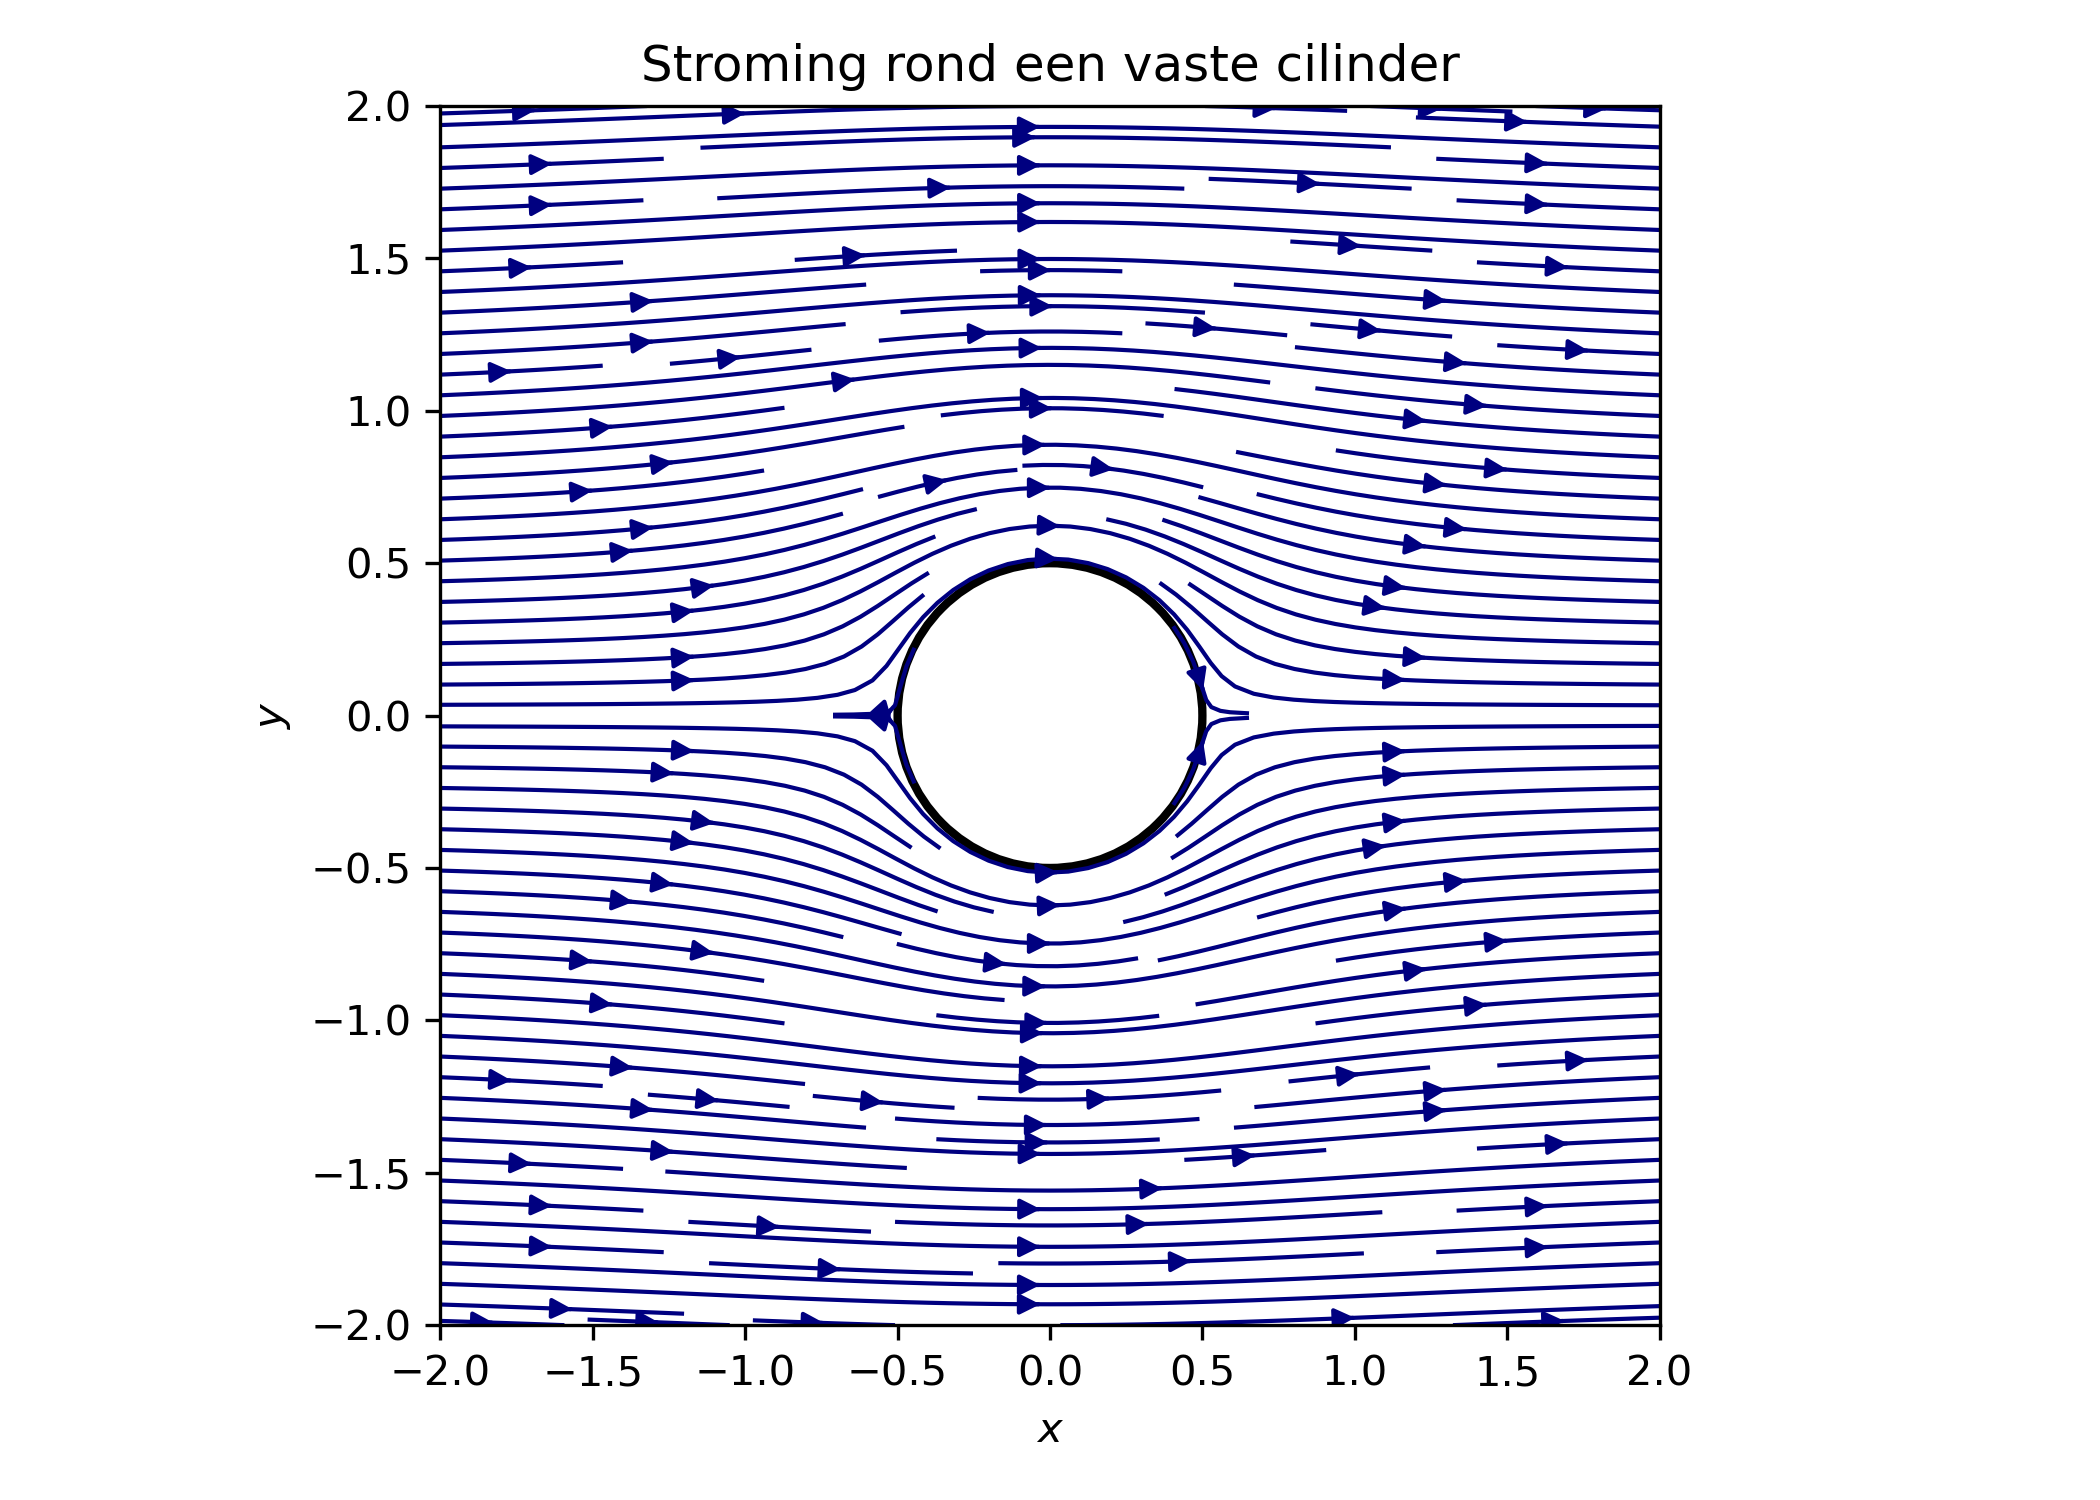
\includegraphics[width=0.85\textwidth]{02_cylinder_flow}
    \caption{Visualisatie van stroming rond een vaste cilinder als analogie voor ætherstroming rond een stabiele wervel in het æthermodel. De uniforme achtergrondstroom wordt lokaal vervormd door de aanwezigheid van de wervelstructuur. Dit klassieke potentiaalstroomprofiel vormt de basis voor latere interpretaties van ætherinteracties in het model.}
    \label{fig:cylinderflow}
\end{figure}

\section{Introductie}
In een moderne heropleving van Lord Kelvins wervel-atoomhypothese uit 1867~\cite{Kelvin1867-vortex} beschouwen we een absolute Euclidische ruimte gevuld met een supervloeibare æther. In dit kader zijn elementaire deeltjes (atomen) stabiele wervelknopen in de æther, en \emph{tijd} wordt geïdentificeerd met de intrinsieke hoekrotatie van deze wervelkernen. De uitdaging is om \emph{tijdsdilatatie}-formules af te leiden die analoog zijn aan die in de speciale en algemene relativiteitstheorie (SR en GR), met behulp van fysieke parameters van de æther (zoals constante dichtheid en fundamentele schalen zoals de Planck-tijd) in plaats van 4D-ruimtetijdgeometrie. We vereisen dat elke nieuwe formule gevestigde relativistische effecten reproduceert - bijvoorbeeld het vertragen van klokken in de buurt van een massief lichaam (gravitationele roodverschuiving) of bij hoge snelheid (speciaal-relativistische tijdsdilatatie) - ondanks het werken in een vlakke 3D-achtergrond.Met andere woorden, de \emph{werveldynamica} van de æther — zoals geïllustreerd in Figuur~\ref{fig:cylinderflow} — moet de 4D-metrische kromming van GR met hoge precisie nabootsen.


Dit rapport ontwikkelt een wiskundig rigoureus model voor tijdsdilatatie in het superfluïde ætherparadigma. We beginnen met het formaliseren van
de belangrijkste aannames van het æthermodel en definiëren hoe de rotatie van een wervel als een fysieke klok dient. Vervolgens leiden we twee
sets tijdsdilatatievergelijkingen af: één voor relatieve beweging (analoog aan SR) en één voor gravitatievelden (analoog aan GR). Tot slot laten we zien dat deze resultaten overeenkomen met standaard relativistische voorspellingen (bijv. gravitationele roodverschuiving, orbitale kloksnelheden) en bespreken we hoe \emph{wervelhoeksnelheid} in de æther de ruimtetijdkromming vervangt als het mechanisme van tijdsdilatatie. We citeren primaire literatuur ter vergelijking en validatie en gebruiken fundamentele constanten (Planck-tijd $t_\textrm{P}$, maximale kracht $F_{\max}$, ætherdichtheid $\rho_{\text{\ae}}$, enz.) om de nieuwe formules in vertrouwde termen uit te drukken.